% Options for packages loaded elsewhere
\PassOptionsToPackage{unicode}{hyperref}
\PassOptionsToPackage{hyphens}{url}
%
\documentclass[
]{article}
\usepackage{lmodern}
\usepackage{amssymb,amsmath}
\usepackage{ifxetex,ifluatex}
\ifnum 0\ifxetex 1\fi\ifluatex 1\fi=0 % if pdftex
  \usepackage[T1]{fontenc}
  \usepackage[utf8]{inputenc}
  \usepackage{textcomp} % provide euro and other symbols
\else % if luatex or xetex
  \usepackage{unicode-math}
  \defaultfontfeatures{Scale=MatchLowercase}
  \defaultfontfeatures[\rmfamily]{Ligatures=TeX,Scale=1}
\fi
% Use upquote if available, for straight quotes in verbatim environments
\IfFileExists{upquote.sty}{\usepackage{upquote}}{}
\IfFileExists{microtype.sty}{% use microtype if available
  \usepackage[]{microtype}
  \UseMicrotypeSet[protrusion]{basicmath} % disable protrusion for tt fonts
}{}
\makeatletter
\@ifundefined{KOMAClassName}{% if non-KOMA class
  \IfFileExists{parskip.sty}{%
    \usepackage{parskip}
  }{% else
    \setlength{\parindent}{0pt}
    \setlength{\parskip}{6pt plus 2pt minus 1pt}}
}{% if KOMA class
  \KOMAoptions{parskip=half}}
\makeatother
\usepackage{xcolor}
\IfFileExists{xurl.sty}{\usepackage{xurl}}{} % add URL line breaks if available
\IfFileExists{bookmark.sty}{\usepackage{bookmark}}{\usepackage{hyperref}}
\hypersetup{
  pdftitle={Building a Spotify Recommendation Model With R},
  pdfauthor={Ed Orlando},
  hidelinks,
  pdfcreator={LaTeX via pandoc}}
\urlstyle{same} % disable monospaced font for URLs
\usepackage[margin=1in]{geometry}
\usepackage{color}
\usepackage{fancyvrb}
\newcommand{\VerbBar}{|}
\newcommand{\VERB}{\Verb[commandchars=\\\{\}]}
\DefineVerbatimEnvironment{Highlighting}{Verbatim}{commandchars=\\\{\}}
% Add ',fontsize=\small' for more characters per line
\usepackage{framed}
\definecolor{shadecolor}{RGB}{248,248,248}
\newenvironment{Shaded}{\begin{snugshade}}{\end{snugshade}}
\newcommand{\AlertTok}[1]{\textcolor[rgb]{0.94,0.16,0.16}{#1}}
\newcommand{\AnnotationTok}[1]{\textcolor[rgb]{0.56,0.35,0.01}{\textbf{\textit{#1}}}}
\newcommand{\AttributeTok}[1]{\textcolor[rgb]{0.77,0.63,0.00}{#1}}
\newcommand{\BaseNTok}[1]{\textcolor[rgb]{0.00,0.00,0.81}{#1}}
\newcommand{\BuiltInTok}[1]{#1}
\newcommand{\CharTok}[1]{\textcolor[rgb]{0.31,0.60,0.02}{#1}}
\newcommand{\CommentTok}[1]{\textcolor[rgb]{0.56,0.35,0.01}{\textit{#1}}}
\newcommand{\CommentVarTok}[1]{\textcolor[rgb]{0.56,0.35,0.01}{\textbf{\textit{#1}}}}
\newcommand{\ConstantTok}[1]{\textcolor[rgb]{0.00,0.00,0.00}{#1}}
\newcommand{\ControlFlowTok}[1]{\textcolor[rgb]{0.13,0.29,0.53}{\textbf{#1}}}
\newcommand{\DataTypeTok}[1]{\textcolor[rgb]{0.13,0.29,0.53}{#1}}
\newcommand{\DecValTok}[1]{\textcolor[rgb]{0.00,0.00,0.81}{#1}}
\newcommand{\DocumentationTok}[1]{\textcolor[rgb]{0.56,0.35,0.01}{\textbf{\textit{#1}}}}
\newcommand{\ErrorTok}[1]{\textcolor[rgb]{0.64,0.00,0.00}{\textbf{#1}}}
\newcommand{\ExtensionTok}[1]{#1}
\newcommand{\FloatTok}[1]{\textcolor[rgb]{0.00,0.00,0.81}{#1}}
\newcommand{\FunctionTok}[1]{\textcolor[rgb]{0.00,0.00,0.00}{#1}}
\newcommand{\ImportTok}[1]{#1}
\newcommand{\InformationTok}[1]{\textcolor[rgb]{0.56,0.35,0.01}{\textbf{\textit{#1}}}}
\newcommand{\KeywordTok}[1]{\textcolor[rgb]{0.13,0.29,0.53}{\textbf{#1}}}
\newcommand{\NormalTok}[1]{#1}
\newcommand{\OperatorTok}[1]{\textcolor[rgb]{0.81,0.36,0.00}{\textbf{#1}}}
\newcommand{\OtherTok}[1]{\textcolor[rgb]{0.56,0.35,0.01}{#1}}
\newcommand{\PreprocessorTok}[1]{\textcolor[rgb]{0.56,0.35,0.01}{\textit{#1}}}
\newcommand{\RegionMarkerTok}[1]{#1}
\newcommand{\SpecialCharTok}[1]{\textcolor[rgb]{0.00,0.00,0.00}{#1}}
\newcommand{\SpecialStringTok}[1]{\textcolor[rgb]{0.31,0.60,0.02}{#1}}
\newcommand{\StringTok}[1]{\textcolor[rgb]{0.31,0.60,0.02}{#1}}
\newcommand{\VariableTok}[1]{\textcolor[rgb]{0.00,0.00,0.00}{#1}}
\newcommand{\VerbatimStringTok}[1]{\textcolor[rgb]{0.31,0.60,0.02}{#1}}
\newcommand{\WarningTok}[1]{\textcolor[rgb]{0.56,0.35,0.01}{\textbf{\textit{#1}}}}
\usepackage{graphicx,grffile}
\makeatletter
\def\maxwidth{\ifdim\Gin@nat@width>\linewidth\linewidth\else\Gin@nat@width\fi}
\def\maxheight{\ifdim\Gin@nat@height>\textheight\textheight\else\Gin@nat@height\fi}
\makeatother
% Scale images if necessary, so that they will not overflow the page
% margins by default, and it is still possible to overwrite the defaults
% using explicit options in \includegraphics[width, height, ...]{}
\setkeys{Gin}{width=\maxwidth,height=\maxheight,keepaspectratio}
% Set default figure placement to htbp
\makeatletter
\def\fps@figure{htbp}
\makeatother
\setlength{\emergencystretch}{3em} % prevent overfull lines
\providecommand{\tightlist}{%
  \setlength{\itemsep}{0pt}\setlength{\parskip}{0pt}}
\setcounter{secnumdepth}{-\maxdimen} % remove section numbering

\title{Building a Spotify Recommendation Model With R}
\author{Ed Orlando}
\date{2020-05-18}

\begin{document}
\maketitle

\hypertarget{author-ed-orlando}{%
\subsubsection{Author: Ed Orlando}\label{author-ed-orlando}}

\hypertarget{problem-statement}{%
\subsubsection{Problem Statement}\label{problem-statement}}

This tutorial shows you how to create a Spotify Recommendation Algorithm
using the \textbf{recommenderlab()} and \textbf{arules()} packages.

\hypertarget{load-libraries}{%
\subsubsection{Load Libraries}\label{load-libraries}}

To get started, first load the libbraries listed below.

\begin{Shaded}
\begin{Highlighting}[]
\CommentTok{# Core & Viz}
\KeywordTok{library}\NormalTok{(tidyverse)}
\KeywordTok{library}\NormalTok{(tidyquant)}
\KeywordTok{library}\NormalTok{(plotly)}

\CommentTok{# Modeling}
\KeywordTok{library}\NormalTok{(recommenderlab)}
\KeywordTok{library}\NormalTok{(arules)}
\CommentTok{#library(arulesViz)}
\end{Highlighting}
\end{Shaded}

\hypertarget{load-data}{%
\subsubsection{Load Data}\label{load-data}}

The data was previously downloaded using
\textbf{\href{https://rawgit.com/watsonbox/exportify/master/exportify.html}{Exportify}}.
There were 27 various genres included and each genre has 10-60 various
playlists included. We will analyze more of this detail later, but
first, let's load the data.

\begin{Shaded}
\begin{Highlighting}[]
\NormalTok{playlist_tbl <-}\StringTok{ }\KeywordTok{read_csv2}\NormalTok{(}\StringTok{"Data_Sources/2020_05_20_Spotify_Playlist_Data/all_playlists.csv"}\NormalTok{)}
\end{Highlighting}
\end{Shaded}

\hypertarget{viewing-the-data}{%
\subsubsection{Viewing the Data}\label{viewing-the-data}}

The data consists of \textbf{\textasciitilde103K songs} and \textbf{18
variables}. You may view the .csv file
\textbf{\href{https://ed-orlando07.netlify.app/zip_files/Spotify_Playlist.zip}{here}}.
The features included in the data set are listed below.

Additional columns, including the genre, playlist, artist/track name
concatenation were all previously engineered. For more information
related to engineering these columns, please visit my previous post
\textbf{\href{https://ed-orlando07.netlify.app/2020/05/14/loading-multiple-files-from-various-folders-in-r/}{here}}.

\begin{Shaded}
\begin{Highlighting}[]
\NormalTok{playlist_tbl }\OperatorTok\StringTok{ }\KeywordTok{glimpse}\NormalTok{()}
\CommentTok{## Observations: 103,517}
\CommentTok{## Variables: 18}
\CommentTok{## $ spotify_uri           <chr> "spotify:track:7EFnbc7UnvOyFcb6IhJq9v", "spot...}
\CommentTok{## $ track_name            <chr> "Oreke", "Know Your Worth", "Don't Rush (feat...}
\CommentTok{## $ artist_name           <chr> "E Kelly, Joeboy", "Khalid, Disclosure, DaVid...}
\CommentTok{## $ album_name            <chr> "No Secrets", "Know Your Worth", "Don't Rush ...}
\CommentTok{## $ disc_number           <dbl> 1, 1, 1, 1, 1, 1, 1, 1, 1, 1, 1, 1, 1, 1, 1, ...}
\CommentTok{## $ track_number          <dbl> 3, 1, 1, 1, 1, 1, 1, 1, 2, 1, 1, 1, 1, 1, 1, ...}
\CommentTok{## $ `track_duration_(ms)` <dbl> 182639, 191067, 207640, 164571, 176962, 19609...}
\CommentTok{## $ added_by              <chr> "spotify:user:", "spotify:user:", "spotify:us...}
\CommentTok{## $ added_at              <dttm> 2020-05-07 21:59:00, 2020-04-24 07:33:23, 20...}
\CommentTok{## $ playlist_name         <chr> "african_heat", "african_heat", "african_heat...}
\CommentTok{## $ filename              <chr> "./00_Data_Sources/Genres_Moods/Afro/african_...}
\CommentTok{## $ dot                   <chr> ".", ".", ".", ".", ".", ".", ".", ".", ".", ...}
\CommentTok{## $ folder_01             <chr> "00_Data_Sources", "00_Data_Sources", "00_Dat...}
\CommentTok{## $ folder_02             <chr> "Genres_Moods", "Genres_Moods", "Genres_Moods...}
\CommentTok{## $ genre                 <chr> "Afro", "Afro", "Afro", "Afro", "Afro", "Afro...}
\CommentTok{## $ playlist              <chr> "african_heat.csv", "african_heat.csv", "afri...}
\CommentTok{## $ artist_track_name     <chr> "E Kelly, Joeboy ||| Oreke", "Khalid, Disclos...}
\CommentTok{## $ source_playlist_id    <chr> "Afro_african_heat", "Afro_african_heat", "Af...}
\end{Highlighting}
\end{Shaded}

\hypertarget{which-genres-have-the-most-playlists}{%
\subsubsection{Which Genres Have the Most
Playlists?}\label{which-genres-have-the-most-playlists}}

Next, we can view which genre's have the highest number of playlists in
the data file using \textbf{ggplot2()}.

\begin{Shaded}
\begin{Highlighting}[]
\NormalTok{genre_frequency_tbl <-}\StringTok{ }\NormalTok{playlist_tbl }\OperatorTok
\StringTok{    }\KeywordTok{count}\NormalTok{(genre) }\OperatorTok
\StringTok{    }\KeywordTok{arrange}\NormalTok{(}\KeywordTok{desc}\NormalTok{(n)) }\OperatorTok
\StringTok{    }\KeywordTok{rowid_to_column}\NormalTok{(}\DataTypeTok{var =} \StringTok{"rank"}\NormalTok{)}

\NormalTok{g_}\DecValTok{00}\NormalTok{ <-}\StringTok{ }\NormalTok{genre_frequency_tbl }\OperatorTok
\StringTok{    }\NormalTok{ggplot2}\OperatorTok{::}\KeywordTok{ggplot}\NormalTok{(}\KeywordTok{aes}\NormalTok{(}\DataTypeTok{x =} \KeywordTok{reorder}\NormalTok{(genre, n), }
                           \DataTypeTok{y    =}\NormalTok{ n, }
                           \DataTypeTok{fill =}\NormalTok{ n)) }\OperatorTok{+}
\StringTok{    }\KeywordTok{geom_bar}\NormalTok{(}\DataTypeTok{stat =} \StringTok{"identity"}\NormalTok{,}
             \DataTypeTok{show.legend =} \OtherTok{FALSE}\NormalTok{) }\OperatorTok{+}
\StringTok{    }\KeywordTok{scale_fill_gradient2}\NormalTok{(}\DataTypeTok{low=}\StringTok{"#000000"}\NormalTok{, }\DataTypeTok{mid=}\StringTok{"#000000"}\NormalTok{, }\DataTypeTok{high=}\StringTok{"#000000"}\NormalTok{) }\OperatorTok{+}
\StringTok{    }\KeywordTok{coord_flip}\NormalTok{() }\OperatorTok{+}
\StringTok{    }\KeywordTok{theme_tq}\NormalTok{() }\OperatorTok{+}
\StringTok{    }\KeywordTok{scale_color_tq}\NormalTok{() }\OperatorTok{+}
\StringTok{    }\KeywordTok{theme}\NormalTok{(}\DataTypeTok{legend.direction =} \StringTok{"vertical"}\NormalTok{, }
          \DataTypeTok{legend.position  =} \StringTok{"right"}\NormalTok{,}
          \DataTypeTok{panel.grid.major.x =} \KeywordTok{element_blank}\NormalTok{(),}
          \DataTypeTok{panel.grid.major.y =} \KeywordTok{element_blank}\NormalTok{(),}
          \DataTypeTok{axis.text.x  =} \KeywordTok{element_text}\NormalTok{(}\DataTypeTok{color=}\StringTok{"#000000"}\NormalTok{),}
          \DataTypeTok{axis.text.y  =} \KeywordTok{element_text}\NormalTok{(}\DataTypeTok{color=}\StringTok{"#000000"}\NormalTok{),}
          \DataTypeTok{axis.title.x =} \KeywordTok{element_blank}\NormalTok{(),}
          \DataTypeTok{axis.title.y =} \KeywordTok{element_blank}\NormalTok{()) }\OperatorTok{+}\StringTok{ }
\StringTok{    }\KeywordTok{labs}\NormalTok{(}\DataTypeTok{title =} \StringTok{"Genre Song Frequency"}\NormalTok{)}

\NormalTok{g_}\DecValTok{00}
\end{Highlighting}
\end{Shaded}

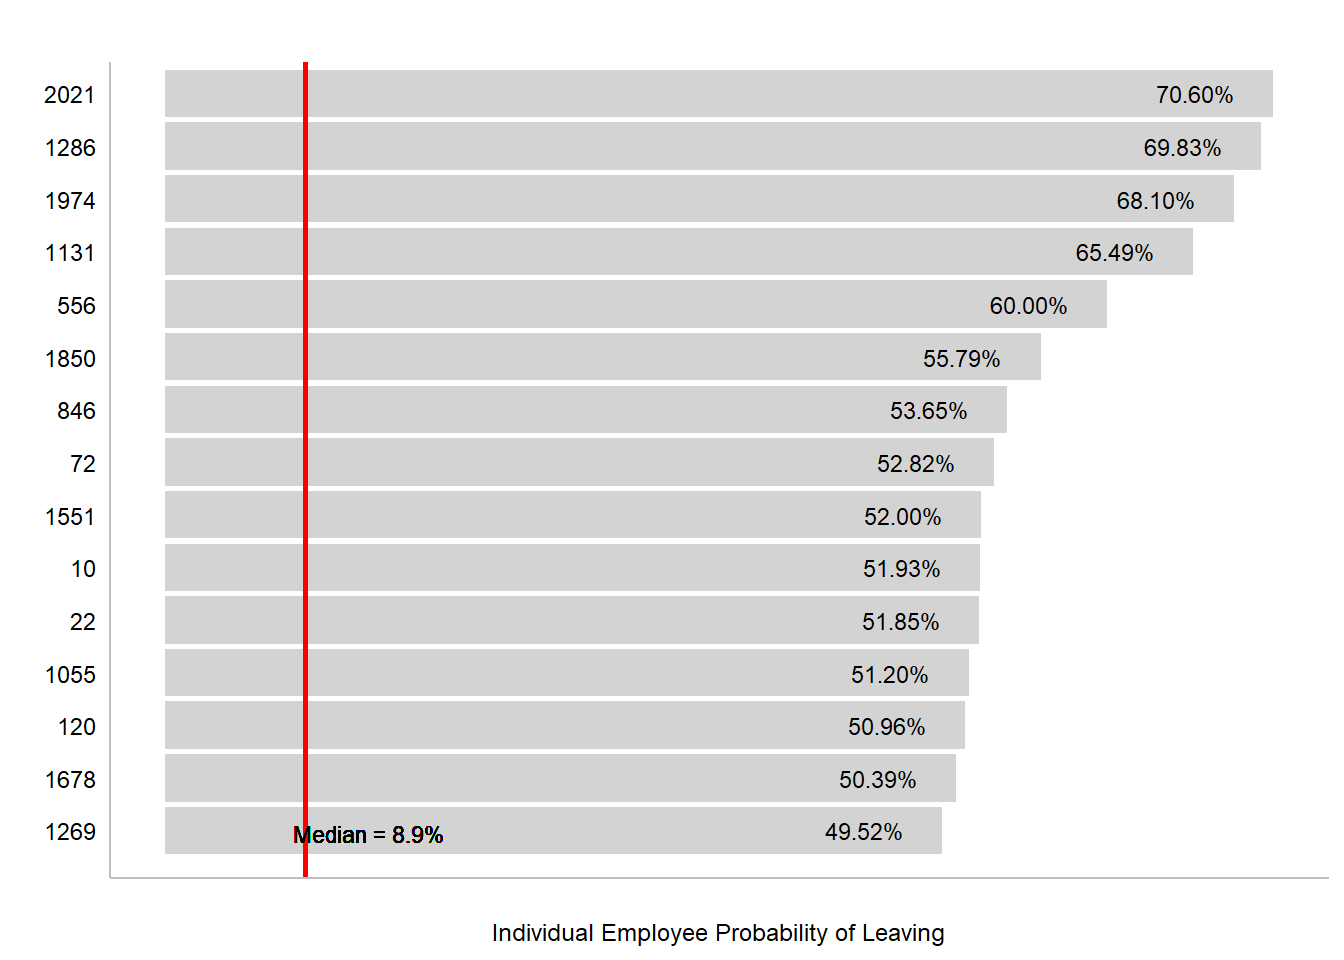
\includegraphics[width=1\linewidth,height=600px]{2020-05-18-Spotify-Recommendation-Algo_files/figure-latex/unnamed-chunk-4-1}

\hypertarget{which-songs-are-the-most-frequent}{%
\subsubsection{Which Songs Are the Most
Frequent?}\label{which-songs-are-the-most-frequent}}

We can also see which songs appear the most in multiple playlists.

\begin{Shaded}
\begin{Highlighting}[]
\NormalTok{song_frequency_tbl <-}\StringTok{ }\NormalTok{playlist_tbl }\OperatorTok
\StringTok{    }\KeywordTok{count}\NormalTok{(artist_name, track_name, artist_track_name) }\OperatorTok
\StringTok{    }\KeywordTok{arrange}\NormalTok{(}\KeywordTok{desc}\NormalTok{(n)) }\OperatorTok
\StringTok{    }\KeywordTok{rowid_to_column}\NormalTok{(}\DataTypeTok{var =} \StringTok{"rank"}\NormalTok{)}

\NormalTok{g_}\DecValTok{01}\NormalTok{ <-}\StringTok{ }\NormalTok{song_frequency_tbl }\OperatorTok
\StringTok{    }\KeywordTok{filter}\NormalTok{(rank }\OperatorTok{<=}\StringTok{ }\DecValTok{10}\NormalTok{) }\OperatorTok\StringTok{ }
\StringTok{    }\KeywordTok{ggplot}\NormalTok{(}\KeywordTok{aes}\NormalTok{(}\DataTypeTok{x =} \KeywordTok{reorder}\NormalTok{(artist_track_name, n), }
                           \DataTypeTok{y    =}\NormalTok{ n, }
                           \DataTypeTok{fill =}\NormalTok{ n)) }\OperatorTok{+}
\StringTok{    }\KeywordTok{geom_bar}\NormalTok{(}\DataTypeTok{stat =} \StringTok{"identity"}\NormalTok{,}
             \DataTypeTok{show.legend =} \OtherTok{FALSE}\NormalTok{) }\OperatorTok{+}
\StringTok{    }\KeywordTok{scale_fill_gradient2}\NormalTok{(}\DataTypeTok{low=}\StringTok{"#000000"}\NormalTok{, }\DataTypeTok{mid=}\StringTok{"#000000"}\NormalTok{, }\DataTypeTok{high=}\StringTok{"#000000"}\NormalTok{) }\OperatorTok{+}
\StringTok{    }\KeywordTok{coord_flip}\NormalTok{() }\OperatorTok{+}
\StringTok{    }\KeywordTok{theme_tq}\NormalTok{() }\OperatorTok{+}
\StringTok{    }\KeywordTok{scale_color_tq}\NormalTok{() }\OperatorTok{+}
\StringTok{    }\KeywordTok{theme}\NormalTok{(}\DataTypeTok{legend.direction =} \StringTok{"vertical"}\NormalTok{, }
          \DataTypeTok{legend.position  =} \StringTok{"right"}\NormalTok{,}
          \DataTypeTok{panel.grid.major.x =} \KeywordTok{element_blank}\NormalTok{(),}
          \DataTypeTok{panel.grid.major.y =} \KeywordTok{element_blank}\NormalTok{(),}
          \DataTypeTok{axis.text.x  =} \KeywordTok{element_text}\NormalTok{(}\DataTypeTok{color=}\StringTok{"#000000"}\NormalTok{),}
          \DataTypeTok{axis.text.y  =} \KeywordTok{element_text}\NormalTok{(}\DataTypeTok{color=}\StringTok{"#000000"}\NormalTok{),}
          \DataTypeTok{axis.title.x =} \KeywordTok{element_blank}\NormalTok{(),}
          \DataTypeTok{axis.title.y =} \KeywordTok{element_blank}\NormalTok{()) }\OperatorTok{+}\StringTok{ }
\StringTok{    }\KeywordTok{labs}\NormalTok{(}\DataTypeTok{title =} \StringTok{"Top 10 Artist/Track Names"}\NormalTok{)}

\NormalTok{g_}\DecValTok{01}
\end{Highlighting}
\end{Shaded}

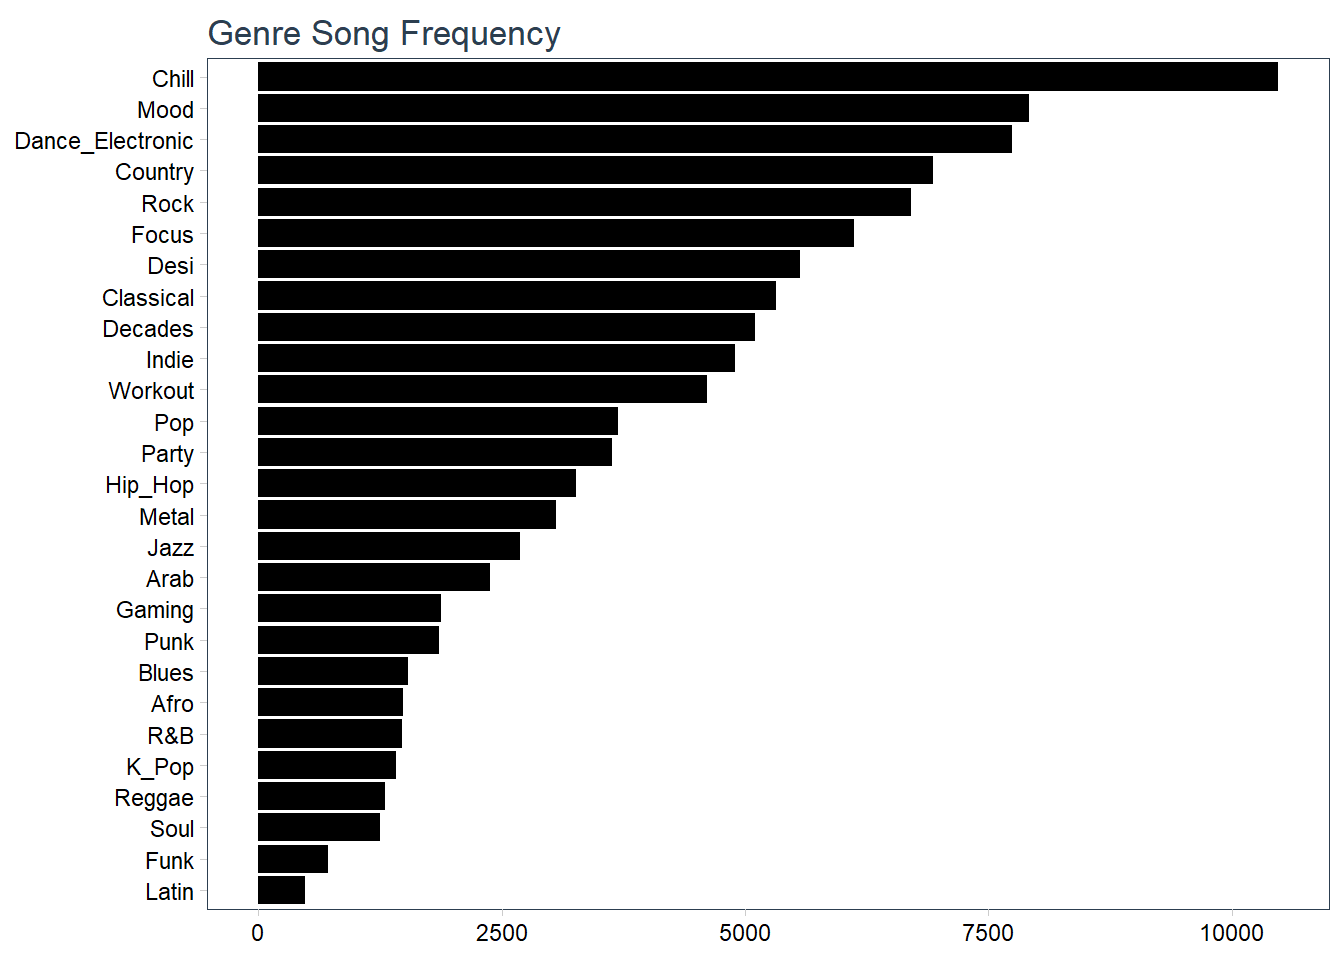
\includegraphics[width=1\linewidth]{2020-05-18-Spotify-Recommendation-Algo_files/figure-latex/unnamed-chunk-5-1}

\hypertarget{condense-the-number-of-songs-in-tibble}{%
\subsubsection{Condense the Number of Songs in
Tibble}\label{condense-the-number-of-songs-in-tibble}}

In order for the Recommendation algorithm to run more efficiently, we
can reduce the number of songs that do not appear at least 3 times.

\begin{Shaded}
\begin{Highlighting}[]
\NormalTok{playlist_condensed_tbl <-}\StringTok{ }\NormalTok{playlist_tbl }\OperatorTok
\StringTok{    }\KeywordTok{left_join}\NormalTok{(song_frequency_tbl) }\OperatorTok
\StringTok{    }\KeywordTok{filter}\NormalTok{(n }\OperatorTok{>=}\StringTok{ }\DecValTok{3}\NormalTok{) }\OperatorTok
\StringTok{    }\KeywordTok{select}\NormalTok{(source_playlist_id, artist_track_name) }\OperatorTok
\StringTok{    }\KeywordTok{distinct}\NormalTok{() }\OperatorTok
\StringTok{    }\KeywordTok{mutate}\NormalTok{(}\DataTypeTok{value =} \DecValTok{1}\NormalTok{) }\OperatorTok
\StringTok{    }\KeywordTok{spread}\NormalTok{(artist_track_name, value, }\DataTypeTok{fill =} \DecValTok{0}\NormalTok{)}
\CommentTok{## Joining, by = c("track_name", "artist_name", "artist_track_name")}

\NormalTok{playlist_song_rlab <-}\StringTok{ }\NormalTok{playlist_condensed_tbl }\OperatorTok
\StringTok{    }\KeywordTok{select}\NormalTok{(}\OperatorTok{-}\NormalTok{source_playlist_id) }\OperatorTok
\StringTok{    }\KeywordTok{as.matrix}\NormalTok{() }\OperatorTok
\StringTok{    }\KeywordTok{as}\NormalTok{(}\StringTok{"binaryRatingMatrix"}\NormalTok{)}
    
\end{Highlighting}
\end{Shaded}

\begin{Shaded}
\begin{Highlighting}[]
\CommentTok{# eval_recipe <- playlist_song_rlab %>%}
\CommentTok{#     evaluationScheme(method = "cross-validation", k = 5, given = -1)}
\CommentTok{# }
\CommentTok{# eval_recipe}
\end{Highlighting}
\end{Shaded}

\begin{Shaded}
\begin{Highlighting}[]
\CommentTok{# algorithms_list <- list(}
\CommentTok{#     "association rules1"  = list(name  = "AR",}
\CommentTok{#                                    param = list(supp = 0.003, conf = 0.70)),}
\CommentTok{#     "association rules2"  = list(name  = "AR",}
\CommentTok{#                                    param = list(supp = 0.003, conf = 0.75)),}
\CommentTok{#     "association rules3"  = list(name  = "AR",}
\CommentTok{#                                   param = list(supp = 0.004, conf = 0.70)),}
\CommentTok{#     "association rules4"  = list(name  = "AR",}
\CommentTok{#                                   param = list(supp = 0.004, conf = 0.75))}
\CommentTok{#  )}
\end{Highlighting}
\end{Shaded}

\begin{Shaded}
\begin{Highlighting}[]
\CommentTok{# !!! }\AlertTok{WARNING}\CommentTok{ - This section is commented out since it is a long-running script !!!}

\CommentTok{# results_rlab_arules <- eval_recipe %>%}
\CommentTok{#     recommenderlab::evaluate(}
\CommentTok{#          method    = algorithms_list,}
\CommentTok{#          type      = "topNList",}
\CommentTok{#          n         = 1:10)}
\end{Highlighting}
\end{Shaded}

\begin{Shaded}
\begin{Highlighting}[]

\CommentTok{# saveRDS(results_rlab_arules, file = "Models/results_arules.rds")}

\NormalTok{results_rlab_arules <-}\StringTok{ }\KeywordTok{read_rds}\NormalTok{(}\StringTok{"Models/results_arules.rds"}\NormalTok{)}

\CommentTok{# plot(results_rlab_arules, annotate = TRUE)}

\NormalTok{arules01_tbl <-}\StringTok{ }\NormalTok{results_rlab_arules}\OperatorTok{$}\StringTok{`}\DataTypeTok{association rules1}\StringTok{`}\OperatorTok{@}\NormalTok{results[[}\DecValTok{1}\NormalTok{]]}\OperatorTok{@}\NormalTok{cm }\OperatorTok\StringTok{ }
\StringTok{    }\KeywordTok{as_tibble}\NormalTok{() }\OperatorTok\StringTok{ }
\StringTok{    }\KeywordTok{mutate}\NormalTok{(}\DataTypeTok{arules_model =} \StringTok{"arules_model_01"}\NormalTok{)}
    
\NormalTok{arules02_tbl <-}\StringTok{ }\NormalTok{results_rlab_arules}\OperatorTok{$}\StringTok{`}\DataTypeTok{association rules2}\StringTok{`}\OperatorTok{@}\NormalTok{results[[}\DecValTok{1}\NormalTok{]]}\OperatorTok{@}\NormalTok{cm }\OperatorTok
\StringTok{    }\KeywordTok{as_tibble}\NormalTok{() }\OperatorTok\StringTok{ }
\StringTok{    }\KeywordTok{mutate}\NormalTok{(}\DataTypeTok{arules_model =} \StringTok{"arules_model_02"}\NormalTok{)}
    
\NormalTok{arules03_tbl <-}\StringTok{ }\NormalTok{results_rlab_arules}\OperatorTok{$}\StringTok{`}\DataTypeTok{association rules3}\StringTok{`}\OperatorTok{@}\NormalTok{results[[}\DecValTok{1}\NormalTok{]]}\OperatorTok{@}\NormalTok{cm }\OperatorTok
\StringTok{    }\KeywordTok{as_tibble}\NormalTok{() }\OperatorTok\StringTok{ }
\StringTok{    }\KeywordTok{mutate}\NormalTok{(}\DataTypeTok{arules_model =} \StringTok{"arules_model_03"}\NormalTok{)}
    
\NormalTok{arules04_tbl <-}\StringTok{ }\NormalTok{results_rlab_arules}\OperatorTok{$}\StringTok{`}\DataTypeTok{association rules4}\StringTok{`}\OperatorTok{@}\NormalTok{results[[}\DecValTok{1}\NormalTok{]]}\OperatorTok{@}\NormalTok{cm }\OperatorTok
\StringTok{    }\KeywordTok{as_tibble}\NormalTok{() }\OperatorTok\StringTok{ }
\StringTok{    }\KeywordTok{mutate}\NormalTok{(}\DataTypeTok{arules_model =} \StringTok{"arules_model_04"}\NormalTok{)}

\NormalTok{arules_combined_tbl <-}\StringTok{ }\KeywordTok{rbind}\NormalTok{(arules01_tbl, arules02_tbl, arules03_tbl, arules04_tbl)}

\NormalTok{arules_combined_tbl }\OperatorTok\StringTok{ }\KeywordTok{glimpse}\NormalTok{()}
\CommentTok{## Observations: 40}
\CommentTok{## Variables: 9}
\CommentTok{## $ TP           <dbl> 0.008333333, 0.012500000, 0.016666667, 0.016666667, 0....}
\CommentTok{## $ FP           <dbl> 0.5708333, 1.1125000, 1.6166667, 2.1041667, 2.5666667,...}
\CommentTok{## $ FN           <dbl> 0.9916667, 0.9875000, 0.9833333, 0.9833333, 0.9833333,...}
\CommentTok{## $ TN           <dbl> 7990.429, 7989.887, 7989.383, 7988.896, 7988.433, 7988...}
\CommentTok{## $ precision    <dbl> 0.014388489, 0.010791367, 0.009592326, 0.007194245, 0....}
\CommentTok{## $ recall       <dbl> 0.008333333, 0.012500000, 0.016666667, 0.016666667, 0....}
\CommentTok{## $ TPR          <dbl> 0.008333333, 0.012500000, 0.016666667, 0.016666667, 0....}
\CommentTok{## $ FPR          <dbl> 7.143453e-05, 1.392191e-04, 2.023109e-04, 2.633171e-04...}
\CommentTok{## $ arules_model <chr> "arules_model_01", "arules_model_01", "arules_model_01...}
\end{Highlighting}
\end{Shaded}

\begin{Shaded}
\begin{Highlighting}[]
\NormalTok{arules_combined_tbl }\OperatorTok\StringTok{ }
\StringTok{    }\KeywordTok{ggplot}\NormalTok{(}\KeywordTok{aes}\NormalTok{(}\DataTypeTok{x=}\NormalTok{FPR, }\DataTypeTok{y=}\NormalTok{TPR, }\DataTypeTok{group=}\NormalTok{arules_model, }\DataTypeTok{color=}\NormalTok{arules_model)) }\OperatorTok{+}
\StringTok{    }\KeywordTok{geom_line}\NormalTok{(}\DataTypeTok{size =} \DecValTok{1}\NormalTok{) }\OperatorTok{+}
\StringTok{    }\KeywordTok{theme_minimal}\NormalTok{() }\OperatorTok{+}
\StringTok{    }
\StringTok{    }\KeywordTok{scale_colour_manual}\NormalTok{(}\DataTypeTok{values =} \KeywordTok{c}\NormalTok{(}\StringTok{"#000000"}\NormalTok{, }\StringTok{"#808080"}\NormalTok{, }\StringTok{"#F08080"}\NormalTok{, }\StringTok{"#DC143C"}\NormalTok{)) }\OperatorTok{+}
\StringTok{    }
\StringTok{    }\CommentTok{#scale_color_tq() +}
\StringTok{    }\KeywordTok{theme}\NormalTok{(}\DataTypeTok{legend.direction =} \StringTok{"vertical"}\NormalTok{, }
          \DataTypeTok{legend.position  =} \StringTok{"right"}\NormalTok{,}
          \DataTypeTok{panel.grid.major.x =} \KeywordTok{element_blank}\NormalTok{(),}
          \DataTypeTok{panel.grid.major.y =} \KeywordTok{element_blank}\NormalTok{(),}
          \DataTypeTok{axis.text.x  =} \KeywordTok{element_text}\NormalTok{(}\DataTypeTok{color=}\StringTok{"#000000"}\NormalTok{),}
          \DataTypeTok{axis.text.y  =} \KeywordTok{element_text}\NormalTok{(}\DataTypeTok{color=}\StringTok{"#000000"}\NormalTok{)) }\OperatorTok{+}
\StringTok{    }\KeywordTok{labs}\NormalTok{(}\DataTypeTok{title =} \StringTok{"A Rules Model Comprarisons"}\NormalTok{)}
\end{Highlighting}
\end{Shaded}

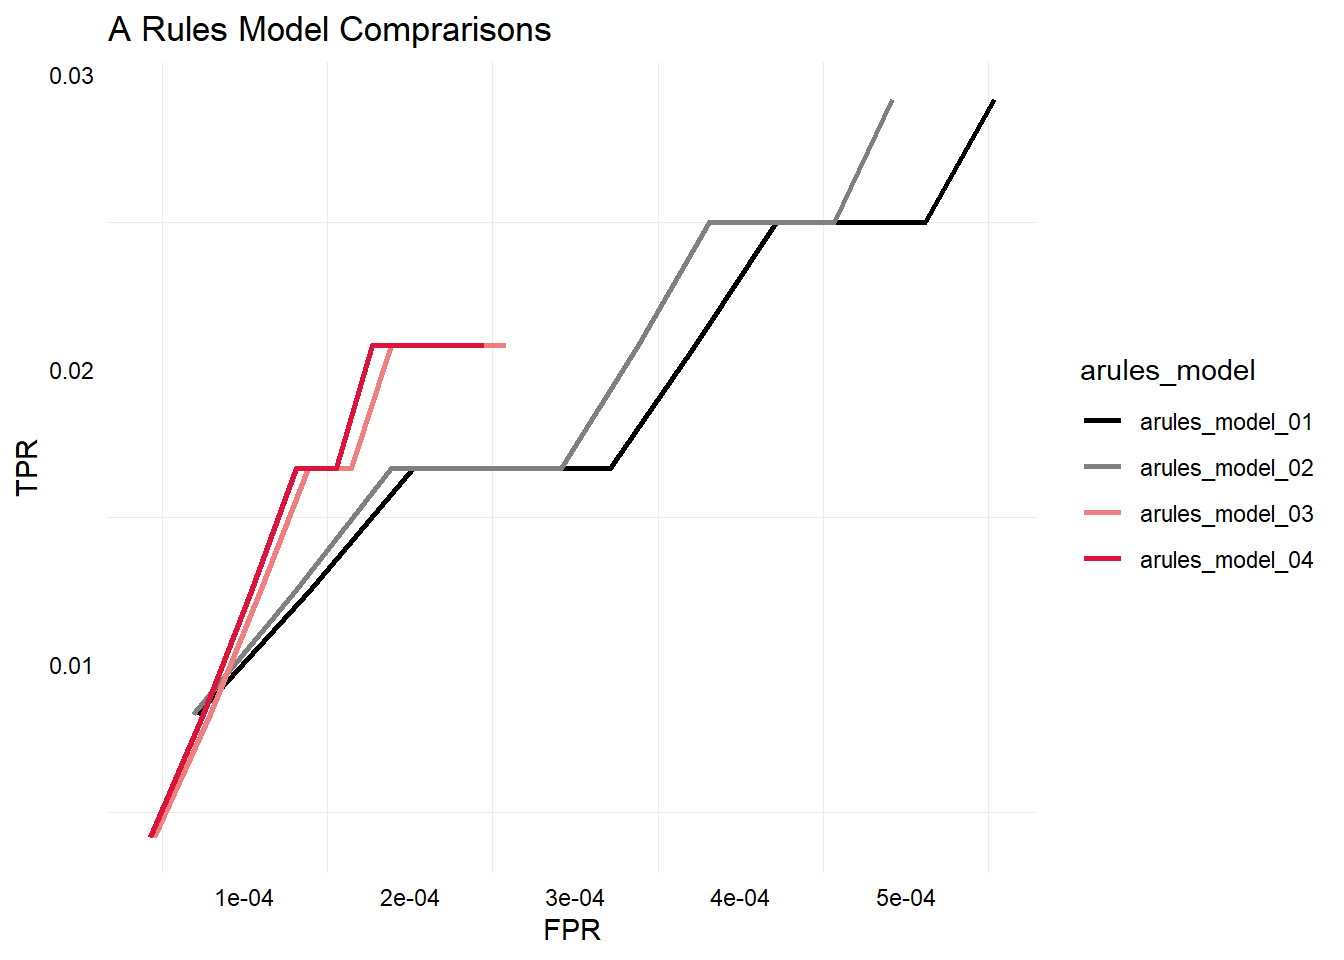
\includegraphics[width=1\linewidth]{2020-05-18-Spotify-Recommendation-Algo_files/figure-latex/unnamed-chunk-11-1}

\end{document}
